\documentclass[12pt,a4paper]{article}
\usepackage{ctex}
\usepackage{amsmath,amscd,amsbsy,amssymb,latexsym,url,bm,amsthm}
\usepackage{epsfig,graphicx,subfigure}
\usepackage{enumitem,balance}
\usepackage{wrapfig}
\usepackage{mathrsfs,euscript}
\usepackage[usenames]{xcolor}
\usepackage{hyperref}
\usepackage[vlined,ruled,commentsnumbered,linesnumbered]{algorithm2e}

\newtheorem{theorem}{Theorem}
\newtheorem{lemma}[theorem]{Lemma}
\newtheorem{proposition}[theorem]{Proposition}
\newtheorem{corollary}[theorem]{Corollary}
\newtheorem{exercise}{Exercise}
\newtheorem*{solution}{Solution}
\newtheorem{definition}{Definition}
\theoremstyle{definition}


%\numberwithin{equation}{section}
%\numberwithin{figure}{section}

\renewcommand{\thefootnote}{\fnsymbol{footnote}}

\newcommand{\postscript}[2]
 {\setlength{\epsfxsize}{#2\hsize}
  \centerline{\epsfbox{#1}}}

\renewcommand{\baselinestretch}{1.0}

\setlength{\oddsidemargin}{-0.365in}
\setlength{\evensidemargin}{-0.365in}
\setlength{\topmargin}{-0.3in}
\setlength{\headheight}{0in}
\setlength{\headsep}{0in}
\setlength{\textheight}{10.1in}
\setlength{\textwidth}{7in}
\makeatletter \renewenvironment{proof}[1][Proof] {\par\pushQED{\qed}\normalfont\topsep6\p@\@plus6\p@\relax\trivlist\item[\hskip\labelsep\bfseries#1\@addpunct{.}]\ignorespaces}{\popQED\endtrivlist\@endpefalse} \makeatother
\makeatletter
\renewenvironment{solution}[1][Solution] {\par\pushQED{\qed}\normalfont\topsep6\p@\@plus6\p@\relax\trivlist\item[\hskip\labelsep\bfseries#1\@addpunct{.}]\ignorespaces}{\popQED\endtrivlist\@endpefalse} \makeatother



\begin{document}
\noindent

%========================================================================
\noindent\framebox[\linewidth]{\shortstack[c]{
\Large{\textbf{Latex Example}}\vspace{1mm}\\
CS214-Algorithm and Complexity, Xiaofeng Gao, Spring 2019}}
\begin{center}
\footnotesize{\color{red}$*$ Please upload your assignment to website. Contact webmaster for any questions.}

\footnotesize{\color{blue}$*$ Name:\_\_\_\_\_\_\_\_\_  \quad Student ID:\_\_\_\_\_\_\_\_\_ \quad Email: \_\_\_\_\_\_\_\_\_\_\_\_}
\end{center}

{\color{purple}Please see the following samples for Latex applications.}

\begin{enumerate}

\item {\color{blue}We use ``enumerate" to list questions. E.g., see this question:} use minimal counterexample principle to prove that for every integer $n>7$, there exist integers $i_n\ge 0$ and $j_n\ge 0$, such that $n = i_n \times 3 + j_n \times 5$.

\begin{proof}
We use ``proof" environment to answer questions asking for \textsc{proof}.
\end{proof}

\item Show that the equation $f(m,n)=2^m(2n+1)-1$ defines a one-to-one correspondence between $\omega \times \omega$ and $\omega$.

\begin{solution}
We use ``solution" environment to answer other questions.
\end{solution}

\item Check how to write in Latex, like:

\begin{itemize}
\item Symbols, like $a$, $b$, $c$, $\alpha$, $\beta$, $\gamma$, $\mathbf{A}$, $\mathbf{B}$, $\mathbf{C}$, $\mathbb{R}$, $\mathbb{S}$, $\mathbb{T}$, $\mathcal{U}$, $\mathcal{V}$, $\mathcal{W}$, $\mathscr{X}$, $\mathscr{Y}$, $\mathscr{Z}$.
\item Functions, like $\sin\theta$, $\max x$, $\lg n$, $\arg \max_i \exp i$.
\item Formulae, like \emph{in-line style} formula $a^2+b^2=c^2$, and \emph{display style} formula $$\sum_{i=1}^n i^2 = \frac{n(n+1)(2n+1)}{6}.$$
\item Environments, like ``enumerate'', ``itemize'', ``definition'', etc.
\end{itemize}

\item Learn Tables and Figures, E.g., fill in the blanks with either true or false:

\begin{table}[h]
	\centering
	\begin{tabular}{|c|c|c|c|c|}
		\hline
		$f(n)$ & $g(n)$ & $f=O(g)$ & $f=\Omega(g)$ & $f=\Theta(g)$ \\
		\hline
		\hline
		$100n^3+3n$ & $100n^2+2n+100$ &  &  & \\
		\hline
		$50n+\log n$ & $10n+\log \log n$ &  &  &  \\
		\hline
		$50n\log^2 n$ & $n \log\log n$ &  &  &  \\
		\hline
		$n^5$ & $3^n$ &  &  &  \\
		\hline
		$n!$ & $5^n$ &  &  &  \\
		\hline
	\end{tabular}
\end{table}

\begin{figure}[htbp]
\begin{minipage}[h]{0.45\textwidth}
\centering
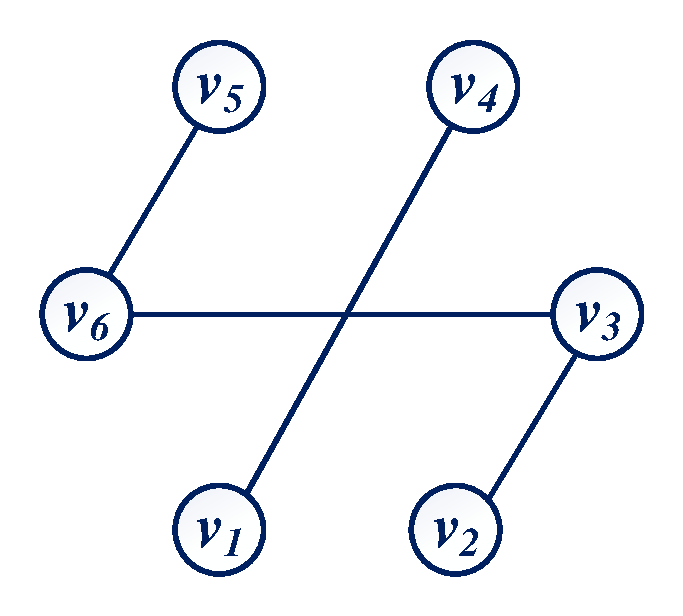
\includegraphics[width=0.5\textwidth]{Fig-GraphG1.pdf}
\caption{Graph $G_1$} \label{Fig-G1}
\end{minipage}
\hspace{5mm}
\begin{minipage}[h]{0.45\textwidth}
\centering
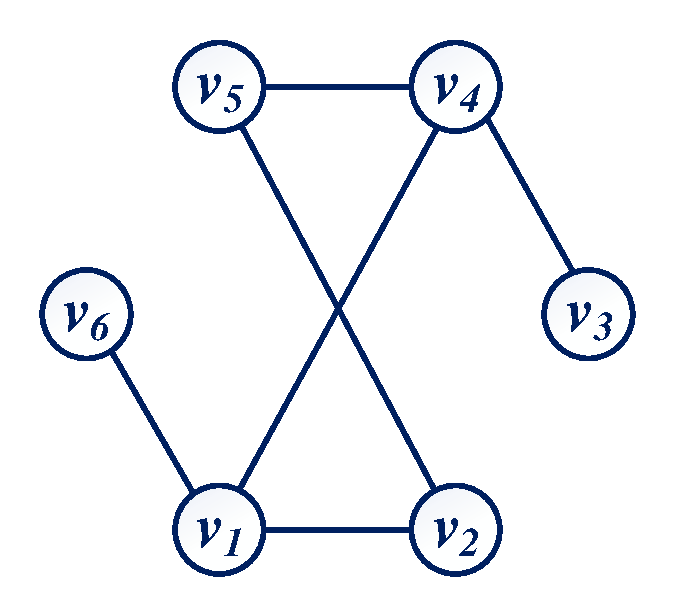
\includegraphics[width=0.5\textwidth]{Fig-GraphG2.pdf}
\caption{Graph $G_2$} \label{Fig-G2}
\end{minipage}
\end{figure}

\item Learn how to use \textbf{algorithm2e} package, like Alg.~\ref{Alg_BUBBLESORT}.

\begin{minipage}[t]{0.9\textwidth}
\begin{algorithm}[H]
	\BlankLine
	\SetKwInOut{Input}{input}
	\SetKwInOut{Output}{output}
	\caption{BUBBLESORT}\label{Alg_BUBBLESORT}
	\Input{An array $A[1\dots n]$ of $n$ elements.}
	\Output{$A[1\dots n]$ in nondecreasing order.}
	\BlankLine
	$i\leftarrow 1;$ $sorted\leftarrow false$\;
	\While{$i\leq n-1$ \textbf{and not} sorted}{
		$sorted \leftarrow true$\;
		\For{$j\leftarrow n$ \textbf{downto} $i+1$}{
			\If{$A[j] < A[j-1]$}{
				interchange $A[j]$ and $A[j-1]$\;
				$sorted\leftarrow false$\;
			}
		}
		$i\leftarrow i+1$\;
	}
	
\end{algorithm}
\end{minipage}
\hspace{2mm}

\begin{enumerate}
	\item What is the minimum number of element comparisons? When is this minimum achieved?
    \begin{solution}
        If having multiple sub-questions, put ``solution" environment inside each subquestion.
    \end{solution}
	
	\item What is the maximum number of element comparisons? When is this maximum achieved?
	
	\item Express the running time of Alg.~\ref{Alg_BUBBLESORT} in terms of the $O$ and $\Omega$ notations.
	
	\item Can the running time of the algorithm be expressed in terms of the
	$\Theta$ notation? Explain.
\end{enumerate}
\end{enumerate}

{\color{purple}\textbf{More examples about algorithm2e (Left $\rightarrow$ source code; Right $\rightarrow$ display in PDF):}}

\begin{enumerate}

\item {\color{blue}\textbf{If} block:}

\begin{minipage}[t]{0.5\textwidth}

\begin{verbatim}
\begin{algorithm}[H]
\KwIn{$x$, $y$}
\KwOut{$sign$}
\BlankLine
\caption{$div(x,y)$} \label{Alg-div}
\If{$rm(x,y)=0$}{
    $sign=1$\;
}
\Else{
    $sign=0$\;
}
\Return{$sign$}\;
\end{algorithm}
\end{verbatim}
\end{minipage}
\hspace{2mm}
\begin{minipage}[t]{0.4\textwidth}
\begin{algorithm}[H]
\KwIn{$x$, $y$}
\KwOut{$sign$}
\BlankLine
\caption{$div(x,y)$} \label{Alg-div}
\eIf{$rm(x,y)=0$}{
    $sign \leftarrow 1$\;
}{
    $sign \leftarrow 0$\;
}
\Return{$sign$}\;
\end{algorithm}
\end{minipage}

\newpage
\item {\color{blue}\textbf{If-ElseIf-Else} block:}

\begin{minipage}[t]{0.5\textwidth}
\begin{verbatim}
\begin{algorithm}[H]
\KwIn{$score$}
\KwOut{Letter Grade}
\BlankLine
\caption{LetterGrade($score$)}
\label{Alg-Score}
\uIf{$score \ge 90$}{
    \textbf{output} $A$\;
}
\uElseIf{$80 \le score < 90$}{
    \textbf{output} $B$\;
}
\Else{
    \textbf{output} $P$\;
}
\end{algorithm}
\end{verbatim}
\end{minipage}
\hspace{2mm}
\begin{minipage}[t]{0.4\textwidth}
\begin{algorithm}[H]
\KwIn{$score$}
\KwOut{Letter Grade}
\BlankLine
\caption{LetterGrade($score$)} \label{Alg-Score}

\uIf{$score \ge 90$}{
    \textbf{output} $A$\;
}
\uElseIf{$80 \le score < 90$}{
    \textbf{output} $B$\;
}
\Else{
    \textbf{output} $P$\;
}
\end{algorithm}
\end{minipage}


\item {\color{blue}\textbf{While} block:}

\begin{minipage}[t]{0.5\textwidth}
\begin{verbatim}
\begin{algorithm}[H]
\KwIn{$x$, $y$}
\KwOut{$x$}
\BlankLine
\While{$x \ge y$}{
$x-=y$\;
}
\textbf{output} $x$\;
\end{algorithm}
\end{verbatim}
\end{minipage}
\hspace{2mm}
\begin{minipage}[t]{0.4\textwidth}
\begin{algorithm}[H]
\KwIn{$x$, $y$}
\KwOut{$x$}
\BlankLine
\caption{$rm(x,y)$} \label{Alg-rm}
\While{$x \ge y$}{
$x-=y$\;
}
\textbf{output} $x$\;
\end{algorithm}
\end{minipage}

\item {\color{blue}\textbf{For} block:}

\begin{minipage}[t]{0.5\textwidth}
\begin{verbatim}
\begin{algorithm}[H]
\KwIn{$n \in \mathbb{N}$}
\KwOut{The sum from 1 to $n$}
\BlankLine
\caption{Sum($n$)} \label{Alg-Sum}
$sum=0$\;
\For{$temp=0$ to $n$}{
    $sum=sum+temp$\;
}
\textbf{output} $sum$\;
\end{algorithm}
\end{verbatim}
\end{minipage}
\hspace{2mm}
\begin{minipage}[t]{0.4\textwidth}
\begin{algorithm}[H]
\KwIn{$n \in \mathbb{N}$}
\KwOut{The sum from 1 to $n$}
\BlankLine
\caption{Sum($n$)} \label{Alg-Sum}
$sum \leftarrow 0$\;
\For{$temp=0$ to $n$}{
    $sum \leftarrow sum+temp$\;
}
\textbf{output} $sum$\;
\end{algorithm}
\end{minipage}

\newpage
\item {\color{blue}\textbf{Repeat-Until} block:}

\begin{minipage}[t]{0.5\textwidth}
\begin{verbatim}
\begin{algorithm}[H]
\KwIn{$a, b \in \mathbb{N}$}
\KwOut{Greatest common divide of $a$, $b$}
\BlankLine
\caption{GCD($a$, $b$)} \label{Alg-GCD}

\Repeat{$gcd=0$}{
    $gcd = a \mod b$\;
    $a=b$\;
    $b=gcd$\;
}
\textbf{output} $gcd$\;
\end{algorithm}
\end{verbatim}
\end{minipage}
\hspace{2mm}
\begin{minipage}[t]{0.4\textwidth}
\begin{algorithm}[H]
\KwIn{$a, b \in \mathbb{N}$}
\KwOut{Greatest common divisor of $a$, $b$}
\BlankLine
\caption{GCD($a$, $b$)} \label{Alg-GCD}

\Repeat{$gcd=0$}{
    $gcd \leftarrow a \mod b$\;
    $a \leftarrow b$\;
    $b \leftarrow gcd$\;
}
\textbf{output} $gcd$\;
\end{algorithm}
\end{minipage}

\item {\color{blue}\textbf{Case} block:}

\begin{minipage}[t]{0.5\textwidth}
\begin{verbatim}
\begin{algorithm}[H]
\KwIn{$person$}
\KwOut{$person$'s gender}
\BlankLine
\caption{Gender} \label{Alg-Gender}
\Switch{$person$}{
\uCase{$person.gender=male$}{
	\textbf{output} Male\;
}
\uCase{$person.gender=female$}{
	\textbf{output} Female\;
}
\Other{
	\textbf{output} Unknown\;
}
}
\end{algorithm}
\end{verbatim}
\end{minipage}
\hspace{2mm}
\begin{minipage}[t]{0.4\textwidth}
\begin{algorithm}[H]
\KwIn{$person$}
\KwOut{$person$'s gender}
\BlankLine
\caption{Gender} \label{Alg-Gender}
\Switch{$person$}{
\uCase{$person.gender=male$}{
	\textbf{output} Male\;
}
\uCase{$person.gender=female$}{
	\textbf{output} Female\;
}
\Other{
	\textbf{output} Unknown\;
}
}
\end{algorithm}
\end{minipage}
\end{enumerate}

%========================================================================
\end{document}
